% Make nice A4 pages for print:
%\usepackage{pgfpages}
%\pgfpagesuselayout{resize to}[a4paper,border shrink=5mm,landscape]

\beamertemplatenavigationsymbolsempty

\setbeamertemplate{bibliography item}[text]

\usepackage[type={CC},modifier={by-sa},version={4.0}]{doclicense}

\usepackage[utf8]{inputenc}
\usepackage{hyperref}
\usepackage{breakurl}
\usepackage{graphicx}
\usepackage{pgfplots}
\usepackage{pgf}
\usepackage{tikz}
\usetikzlibrary{positioning}
\usetikzlibrary{arrows}
\usetikzlibrary{decorations.markings}
\usetikzlibrary{calc}
\usetikzlibrary{matrix}
\usetikzlibrary{shapes}
\usetikzlibrary{decorations.pathmorphing}
\usetikzlibrary{fit}
\usetikzlibrary{backgrounds}
\usetikzlibrary{plotmarks}
\usepackage{stmaryrd}
\usepackage{listings}
\usepackage{pdflscape}
\usepackage{perpage}
\usepackage{appendixnumberbeamer}

%\usepackage[thmmarks,amsmath,amsthm]{ntheorem} % already included in beamer
\usepackage{thm-restate}

\usepackage[sort&compress,numbers]{natbib}  % to be have \citet, \citeauthor, \citeyear

\MakePerPage{footnote}

\tikzstyle{o}=[r,ppBlue]
\tikzstyle{r}=[thick,rectangle,align=center]
\tikzstyle{t}=[r,ppTrans] %,font=\bfseries]
\tikzstyle{dd}=[densely dashed]
\tikzstyle{n}=[r,ppBlue]
\tikzstyle{p}=[r,ppRed]
\tikzstyle{ppRed}  =[draw=red,  fill=  red!20]
\tikzstyle{ppBlue} =[draw=blue, fill= blue!20]
\tikzstyle{ppGreen}=[draw=green,fill=green!20]
\tikzstyle{ppTrans}=[draw=none, fill=none]

\usetheme{Warsaw}

\useoutertheme[subsection=true]{smoothbars}
%\useoutertheme[subsection=false]{miniframes}

\definecolor{bblue}{HTML}{D7DF01}	% yellow-ish actually, for better black/white printing
\definecolor{rred}{HTML}{C0504D}
\definecolor{ggreen}{HTML}{9BBB59}
\definecolor{ppurple}{HTML}{9F4C7C}
\definecolor{lightgray}{rgb}{0.3,0.3,0.3}
\definecolor{lightergray}{rgb}{0.9,0.9,0.9}
\definecolor{UniBlue}{RGB}{83,121,170}

\DeclareTextFontCommand\textintro{\normalfont\bfseries\itshape} % nice!
\newcommand{\intro}[2][]
{%
	\textintro{#2}%
}
\newcommand{\empha}[2][]
{%
	\emph{#2}%
}

%\theoremstyle{plain}
\newcounter{reqcounter}
\newtheorem{requirement}[reqcounter]{Requirement}

%setbeamercolor{structure}{fg=violet}

\makeatletter
\def\th@task{%
    \normalfont % body font
    \setbeamercolor{block title example}{bg=orange,fg=white}
    \setbeamercolor{block body example}{bg=orange!20,fg=black}
    \def\inserttheoremblockenv{exampleblock}
  }
\makeatother

\theoremstyle{task}
\newtheorem{task}{Task}

\newenvironment{assignment}%
{%\setbeamercolor{background canvas}{bg=violet}%
%\setbeamercolor{structure}{fg=cyan!90!black}%
 \setbeamercolor{frametitle}{bg=orange,fg=white}
\begin{frame}}%
{\end{frame}}%

\AtBeginSection[]{
  \begin{frame}
  \vfill
  \centering
  \begin{beamercolorbox}[sep=8pt,center,shadow=true,rounded=true]{title}
    \usebeamerfont{title}\insertsectionhead\par%
  \end{beamercolorbox}
  \tableofcontents
  \vfill
  \end{frame}
}




\pgfplotsset{compat=1.14}
\author{Markus Raab}


\date{13.01.2021}

\begin{document}

\renewcommand{\enquote}[1]{\emph{``#1''}} % Cannot be done earlier

%%%%%%%%%%%%%%%%%%%%%%%%%%%%%%%
\begin{frame}
	\titlepage
	\doclicenseThis
\end{frame}

%%%%%%%%%%%%%%%%%%%%%%%%%%%%%%%%%%%%%%%%%% 
\section{Background}
{
\shadowcolor{black}
\shadowoffset{0.5pt}
\usebackgroundtemplate{\includegraphics[width=\paperwidth]{pics/clouds.jpg}}%
\begin{frame}
	\frametitle{\shadowtext{Misconfiguration}}
	\begin{itemize}[<+->]
		\item   \textcolor{white}{\shadowtext{\empha[misconfiguration]{misconfigurations}~\cite{yin2011empirical,su2007autobash,attariyan2010automating,xu2015systems} are a major cause}}\\
			\textcolor{white}{\shadowtext{of system failures~\cite{wool2004quantitative,oppenheimer2003internet,pertet2005causes}}}
		\item   \textcolor{white}{\shadowtext{much time is needed to fix misconfigurations~\cite{rabkin2011static,oppenheimer2003internet,yin2011empirical,mahajan2002bgp}}}
	\end{itemize}
\end{frame}
}

\begin{frame}
	\frametitle{Elektra~\cite{raab2016elektra}}
	\begin{itemize}[<+->]
	%	\item \citet{holland2001nofutz}~defined \empha{futzing} to denote \enquote{tinkering or fiddling experimentally}
	%	\item With \intro[no-futz computing]{no-futz computing} \citet{holland2001nofutz} mean \enquote{that futzing should be allowed, but should never be required}
		\item \intro{configuration specification languages} mitigate misconfigurations
		\item \elektra{} is a framework implementing a modular \intro{configuration specification language} for configuration settings
	%	\item In \elektra{} we use properties to specify configuration settings and configuration access
		\item \elektra{} enables \intro[no-futz computing]{no-futz computing} \cite{holland2001nofutz},
			i.e., error-prone \enquote{tinkering or fiddling experimentally} \enquote{should be allowed, but should never be required}
	\end{itemize}
\end{frame}

\begin{frame}
	\frametitle{Requirements of Elektra~\cite{raab2017challenges}}

	\begin{itemize}
		\item extensible and flexible
		\item external to applications
		\item open for introspection
	\end{itemize}
\end{frame}

\section{Elektra}

\begin{frame}
	\frametitle{Metalevels}
	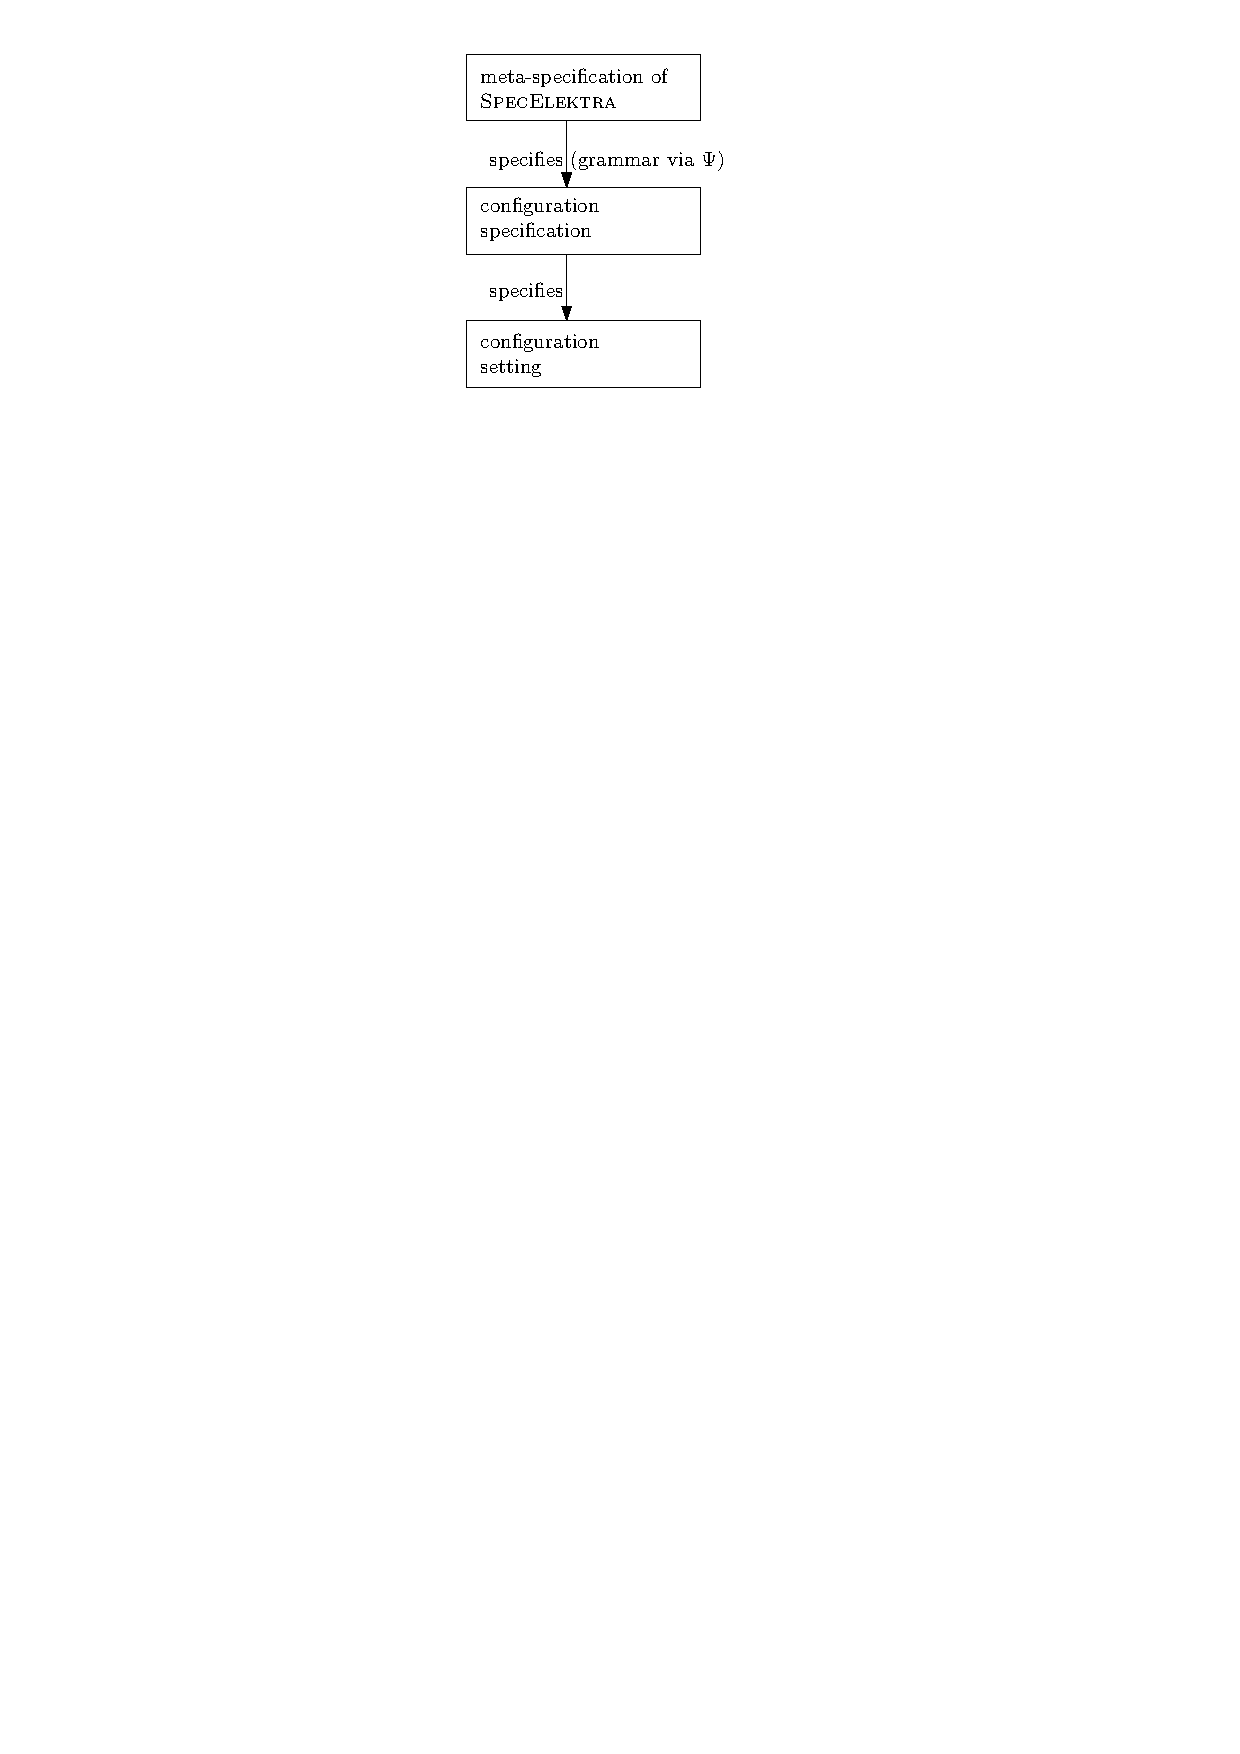
\includegraphics{metalevels}

	We will now walk through metalevels bottom-up.
\end{frame}

\begin{frame}[fragile]
	\frametitle{Configuration Settings}

	A configuration file may look like (properties format):

	\begin{code}[language=CfgElektra]
	slapd/threads/listener=4
	\end{code}

	\vspace{1cm}

	We apply these configuration settings imperatively using:

	\begin{code}[language=bash]
	kdb set /slapd/threads/listener 4
	\end{code}
\end{frame}

\begin{frame}[fragile]
	\frametitle{Specifications}
	For specifications such as:

	\begin{code}
	[slapd/threads/listener]
	  check/range:=1,2,4,8,16
	  default:=1
	  visibility:=advanced
	  description:=One thread is adequate\
		       for up to 16 CPU cores.
	\end{code}

	\vspace{0.6cm}

	We apply the specifications imperatively using:

	\begin{code}[language=bash,morekeywords={meta-set}]
	kdb meta-set /slapd/threads/listener\
		check/range 1,2,4,8,16
	kdb meta-set /slapd/threads/listener\
		default 1
	\end{code}
\end{frame}

\begin{frame}[fragile]
	\frametitle{Meta-Specifications}
	For meta-specifications such as:

	\small
	\begin{code}
	[visibility]
	type:=enum critical important user\
	      advanced developer debug disabled
	description:=Who should see this\
	     configuration setting?
	\end{code}

	\vspace{1cm}

	We apply the meta-specifications imperatively using:

	\begin{code}[language=bash,morekeywords={meta-set}]
	kdb meta-set /elektra/meta/\
		visibility type enum ...
	kdb meta-set /elektra/meta/\
		visibility description "Who ...
	\end{code}
\end{frame}


\begin{frame}[fragile]
	\frametitle{Grammar}
	\begin{alertblock}{Idea}
	Use configuration file format grammar to describe both configurations and (meta-)specifications
	\end{alertblock}

	\begin{grammar}
	<KeySet> ::= \lq ksNew'\WhiteSpace(' \{ <Key> \lq , \LineBreak'  \}  \{ \lq\WhiteSpace' \} \lq KS\_END);'

	<Key> ::= \lq keyNew \WhiteSpace ('' ' <key name> \lq ''  , \LineBreak' [ <Value> ] <properties> \lq KEY_END)'

	<Value> ::=  \{ \lq\WhiteSpace' \} \lq KEY\_VALUE, \WhiteSpace '' ' <configuration value> \lq ''  , \LineBreak'

	<properties> ::= \{ \{ \lq\WhiteSpace' \} <property> \lq , \LineBreak' \}

	<property> ::=  \lq KEY\_META, \WhiteSpace " ' <property name> \lq "  , \WhiteSpace " ' <property value> \lq " '
	\end{grammar}
\end{frame}

\begin{frame}[fragile]
	\frametitle{Example}
	\begin{example}
	Given the key ^/slapd/threads/listener^, with the configuration value ^4^ and the property $\property{default} \mapsto 1$, \elektra{} emits:

	\begin{code}[gobble=4,language=Cpp]
	ksNew (keyNew ("/slapd/threads/listener",
		       KEY_VALUE, "4",
		       KEY_META, "default", "1",
		       KEY_END),
	       KS_END);
	\end{code}
	\vspace{-1em}
	\end{example}

	\pause
	\begin{alertblock}{Finding}
	We have source code representing the settings.
	If we instantiate it, we get a data structure representing the settings.
	Plugins emitting such ``configuration files'' are code generators.
	\end{alertblock}
\end{frame}

\begin{frame}[fragile]
	\frametitle{Usage in Applications}

	With the specification:
	\par
	\begin{code}[gobble=4]
	[slapd/threads/listener]
	  check/range:=1,2,4,8,16
	  default:=1
	  visibility:=advanced
	  restrict/write:=1
	\end{code}
	\par
	\elektra{Gen} gives the user read-only access to the object ^env.slapd.threads.listener^:
	\par
	\begin{code}[language=Cpp]
	std::cout << env.slapd.threads.listener;
	env.slapd.threads.listener = 3; // error
	\end{code}
	\par
\end{frame}

\begin{frame}
	\frametitle{Implementation}
	\begin{columns}[c]
	\begin{column}{6cm}
	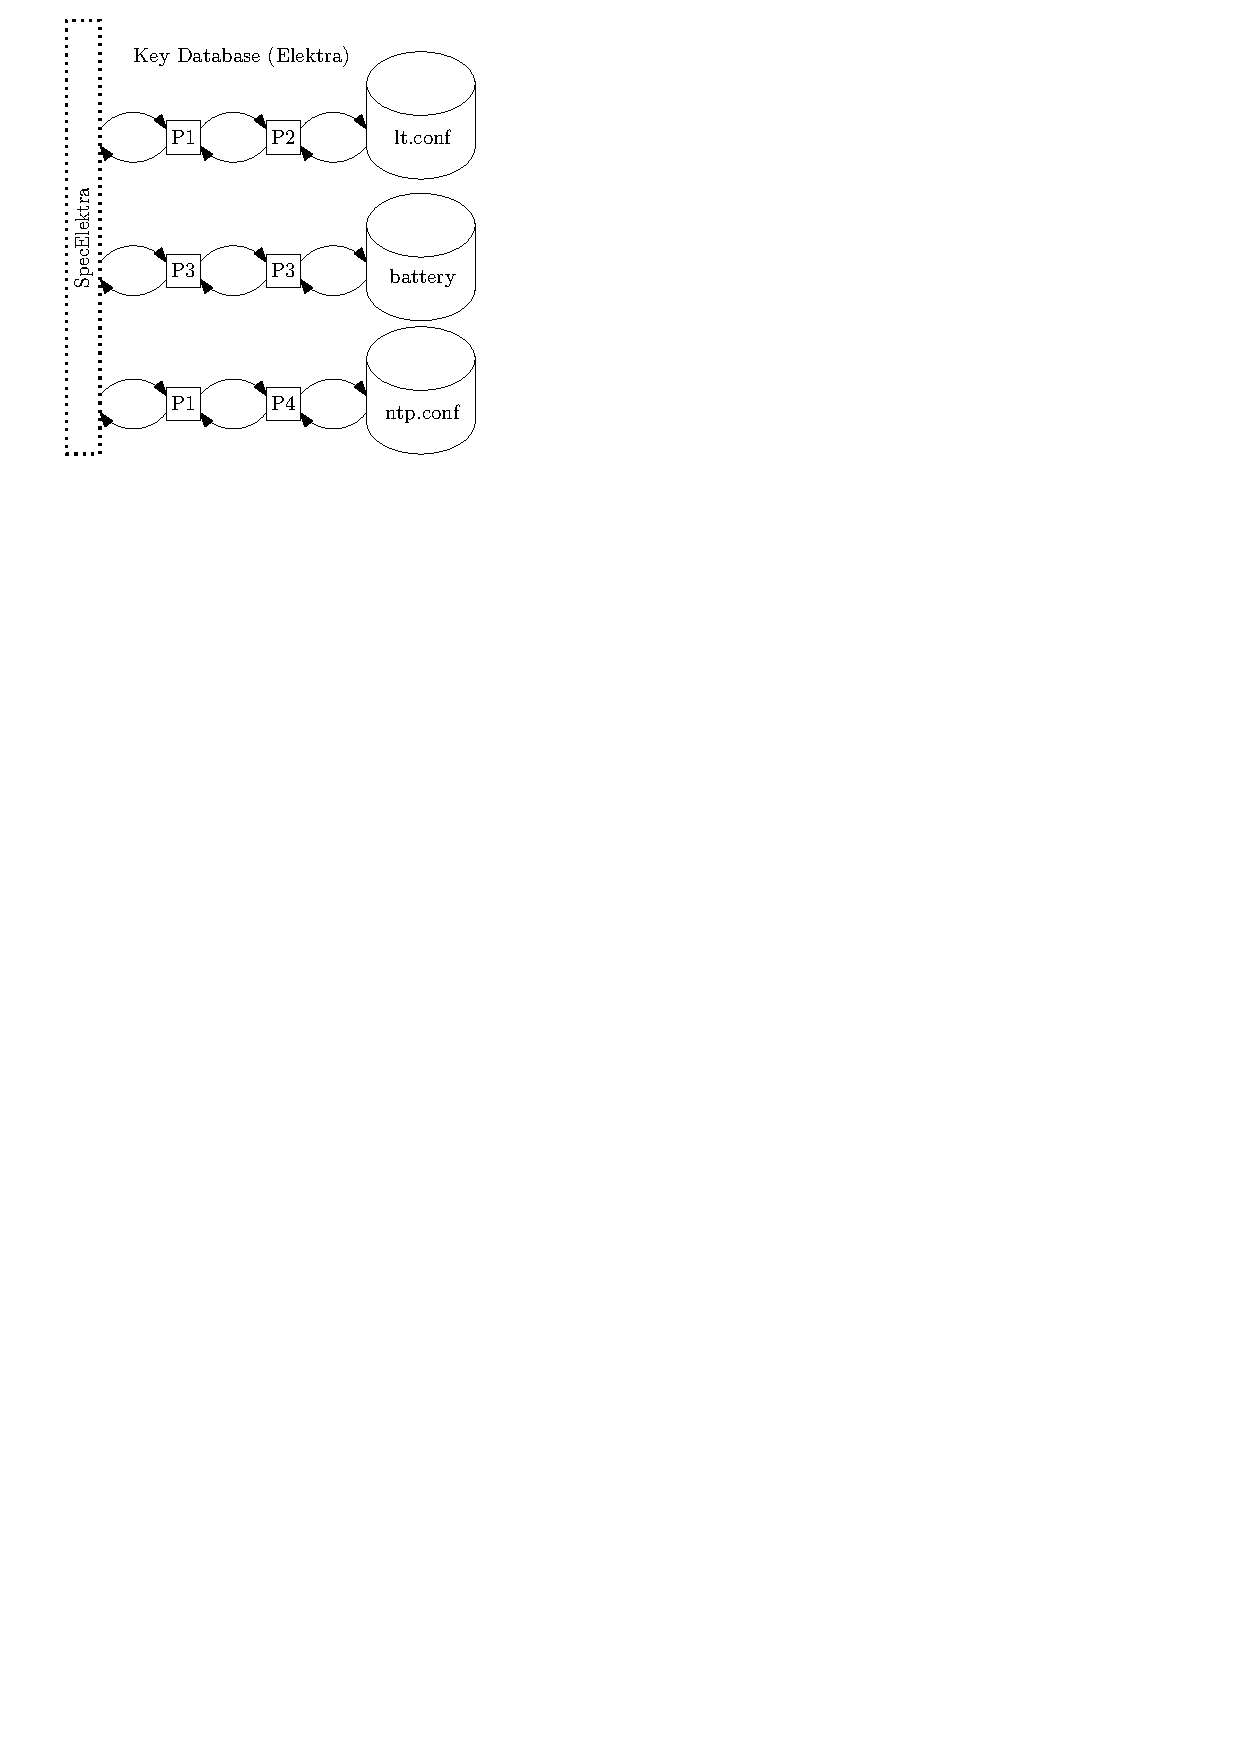
\includegraphics[scale=0.8]{horizontalmodularity}
	\end{column}
	\begin{column}{5cm}
	Cylinders are configuration files, P? are plugins~\cite{raab2016improving}.

	\begin{itemize}
	\item syntax is defined via plugins reading/writing configuration files
	\item semantics are defined via
		\begin{itemize}
		\item plugins interpreting properties
		\item generated code used by applications
		\end{itemize}
	\end{itemize}
	\end{column}
	\end{columns}
\end{frame}

%%%%%%%%%%%%%%%%%%%%%%%%%%%%%%%%%%%%%%%%%% 
\section{Configuration Management}

\begin{frame}[fragile]
	Key/value access in Chef:
	\vspace{0.5cm}

	\begin{code}[morekeywords={kdbset,do,action,value,end},gobble=4]
	kdbset '/slapd/threads/listener' do
		value '4'
		action :create
	end
	\end{code}

	\pause
	\begin{alertblock}{Finding}
	We have CM code representing the settings.
	\end{alertblock}
\end{frame}

\begin{frame}[fragile]
	Key/value access in Ansible:
	\vspace{0.5cm}

	\begin{code}[morekeywords={name,connection,key,value,elektra,mountpoint,file,plugins,hosts,tasks},gobble=4]
	- name: setup LDAP
	  connection: local
	  hosts: localhost
	  tasks:
	  - name: set listening threads
	    elektra:
	      key: '/slapd/threads/listener'
	      value: '4'
	\end{code}
\end{frame}

\begin{frame}[fragile]
	Key/value access in puppet-libelektra~\cite{raab2020unified}:
	\vspace{0.5cm}

	\begin{code}[morekeywords={kdbkey,kdbmount,ensure,value},gobble=4]
	kdbkey {'/slapd/threads/listener':
		ensure => 'present',
		value => '4'
		check => {
			'type' => 'short',
			'range' => '1,2,4,8,16',
			'default' => '1'
		}
	}
	\end{code}
\end{frame}


%%%%%%%%%%%%%%%%%%%%%%%%%%%%%%%%%%%%%%%%%%%%%%%%%%%%
\section{Problems with Flexibility}

\subsection{Feature Interaction}

\begin{frame}[fragile]
	\frametitle{Fixed Order}

	\begin{code}
	[foo/bar]
	  encrypt:=1
	  zip:=1
	\end{code}

	\begin{itemize}
	\item zip must happen before encrypt
	\item must be specified within plugins
	\end{itemize}
\end{frame}

\begin{frame}[fragile]
	\frametitle{Plugins}

	Plugins that modify the KeySet can be very problematic, e.g. notification:
	\begin{code}[gobble=4]
	[foo/bar]
	  rename/toupper:=1
	  notify:=1
	  type:=string
	\end{code}

	\begin{itemize}
	\item expected: notify on change of key
	\item actual: always notifies because of renaming
	\item ordering does not help, as notification must happen at end
	\end{itemize}
\end{frame}

\begin{frame}[fragile]
	\frametitle{Plugins}

	Or even plain contradicting, e.g. assignment:
	\begin{code}[gobble=4]
	[foo/bar]
	  assign/math:=1+1
	  assign/python:=1+2
	  type:=long
	\end{code}

	\begin{alertblock}{Open Question}
	How to deal with it?
	\end{alertblock}
\end{frame}


\subsection{Integration of Operators}

\begin{frame}[fragile]
	\frametitle{In C++/RelaxNG Style}

	\begin{code}[morekeywords={check,type,range,math},gobble=4]
	[t/a]
	type:=long
	restrict/write:=1
	[t/x]
	check/enum/#0:=a
	check/enum/#1:=b
	check/enum/#2:=c
	\end{code}

	could be rendered by a storage plugin by:

	\begin{code}[language=C++,morekeywords={@NonNull,@ReadOnly,string},gobble=4]
	t {
		@restrict/write long a;
		enum {a,b,c} x;
	};
	\end{code}
\end{frame}


\begin{frame}[fragile]
	\frametitle{Types}

	\begin{code}[morekeywords={check,type,range,math},gobble=4]
	[a]
	  check/type:=long
	[b]
	  check/type:=long
	[c]
	  check/type:=long
	  check/range:=0-10
	  check/math:="== + a b"
	\end{code}

	ideal to further restrict types
\end{frame}

\begin{frame}[fragile]
	\frametitle{Integration}

	\begin{code}[morekeywords={check,type,range,math},gobble=4]
	[c]
	  check/type:=long
	  check/range:=0-10
	  check/math:="== + a b"
	  check/condition:="(a == '3') ? (b == '5')"
	\end{code}

	\begin{itemize}
	\item does not allow math expression to be embedded in condition
	\item temporary variables are needed
	\end{itemize}

	\begin{alertblock}{Open Question}
	How to deal with it?
	\end{alertblock}
\end{frame}


\section{Conclusion}

\begin{frame}
	\frametitle{Conclusion}
	\begin{itemize}
	\item Elektra makes configuration management tasks simpler
	\item syntax flexible but limited to key/value formats
	\item plugin development needs careful consideration of interactions
	\item syntax of operators not always combinable
	\end{itemize}
\end{frame}



%%%%%%%%%%%%%%%%%%%%%%%%%%%%%%%%%%%%%%%%%% 
\nocite{raab2017introducing}

\appendix

\begin{frame}[allowframebreaks]
	\bibliographystyle{plainnat}
	\bibliography{../shared/elektra.bib}
\end{frame}

\end{document}


